\documentclass[]{tufte-handout}

% ams
\usepackage{amssymb,amsmath}

\usepackage{ifxetex,ifluatex}
\usepackage{fixltx2e} % provides \textsubscript
\ifnum 0\ifxetex 1\fi\ifluatex 1\fi=0 % if pdftex
  \usepackage[T1]{fontenc}
  \usepackage[utf8]{inputenc}
\else % if luatex or xelatex
  \makeatletter
  \@ifpackageloaded{fontspec}{}{\usepackage{fontspec}}
  \makeatother
  \defaultfontfeatures{Ligatures=TeX,Scale=MatchLowercase}
  \makeatletter
  \@ifpackageloaded{soul}{
     \renewcommand\allcapsspacing[1]{{\addfontfeature{LetterSpace=15}#1}}
     \renewcommand\smallcapsspacing[1]{{\addfontfeature{LetterSpace=10}#1}}
   }{}
  \makeatother

\fi

% graphix
\usepackage{graphicx}
\setkeys{Gin}{width=\linewidth,totalheight=\textheight,keepaspectratio}

% booktabs
\usepackage{booktabs}

% url
\usepackage{url}

% hyperref
\usepackage{hyperref}

% units.
\usepackage{units}


\setcounter{secnumdepth}{-1}

% citations
\usepackage{natbib}
\bibliographystyle{plainnat}

% pandoc syntax highlighting

% longtable

% multiplecol
\usepackage{multicol}

% strikeout
\usepackage[normalem]{ulem}

% morefloats
\usepackage{morefloats}


% tightlist macro required by pandoc >= 1.14
\providecommand{\tightlist}{%
  \setlength{\itemsep}{0pt}\setlength{\parskip}{0pt}}

% title / author / date
\title{Recommended measures to reduce business flights at Eawag}
\author{Flyaware interest group}
\date{2019-11-28}


\begin{document}

\maketitle




\hypertarget{a-call-for-action}{%
\section{A call for action}\label{a-call-for-action}}

\begin{quote}
``It is critical to immediately begin reducing net CO2 emissions and to
eliminate them to zero worldwide between 2040 and 2050 at the latest.''

\hfill --- Scientists for future
\end{quote}

This statement from the `Scientists for Future'\footnote{\url{https://www.scientists4future.org/statement-en-und-es/}}
initiative was signed by 44 out of 87 (50.6\%) Eawag group leaders and
department heads. The director and deputy director of Eawag have signed
this statement as well. Thus, the majority of the Eawag leadership is in
agreement with this statement and is aware of the urgency of taking
measures to reduce emissions.

One of the most effective ways for scientific institutions to reduce
their climate impact is a drastic reduction of business flights. More
than half of greenhouse gas emissions (GHGs) of Eawag's sister
institution ETH Zurich are caused by business trips. Of those
\textbf{93\%} are due to business flights \footnote{\url{https://ethz.ch/flugreisen}}.
Technical alternatives to substantially reduce GHG emissions of
airplanes are not foreseeable for the near future. It is thus of
immediate concern to reduce the number of flights.

Eawag is a research institution recognized worldwide and therefore has
the potential to act as a role model for other research institutes by
taking on its institutional responsibility for further reducing CO2
emissions.

This report is a call to the Eawag leadership to act. We propose nine
concrete sets of measures to reduce Eawag's CO2 emissions related to
business flights. To aid in decision-making, We provide a list of highly
accepted and highly impactful measures as priority targets for
implementation.

\begin{marginfigure}
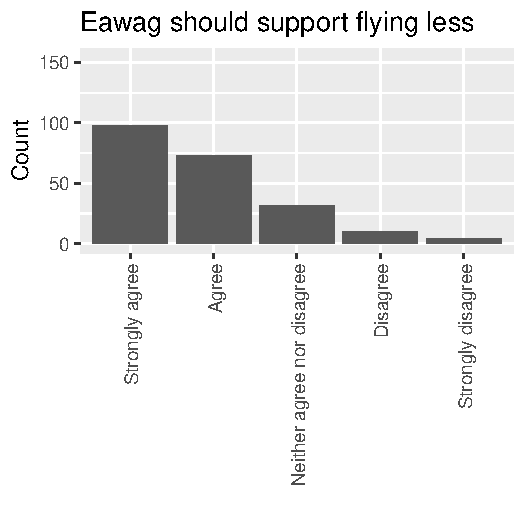
\includegraphics{final_report_files/figure-latex/fig-margin-1} \caption[Employees of Eawag overwhelmingly support Eawag taking measures to aid in reducing business flights]{Employees of Eawag overwhelmingly support Eawag taking measures to aid in reducing business flights}\label{fig:fig-margin}
\end{marginfigure}

We conducted a survey among all Eawag employees, in which roughly half
of all employees (232) participated. Employees were asked to evaluate
the set of measures we present in this report. Given the high response
rate, our results are highly likely to adequately reflect the views of
Eawag employees on the topic of flying and the proposed measures.

The scientific evidence for man-made climate change and its dangers is
robust. We believe that you as (environmental) scientists and members of
the directorate want to overcome the knowledge -- action gap and support
change here at Eawag.

\hypertarget{what-measures-should-eawag-take}{%
\subsection{What measures should Eawag
take?}\label{what-measures-should-eawag-take}}

We suggest the following list of measures for Eawag to take right away.
\footnote{The complete set of measures as presented to Eawag employees
  in the survey can be found at the end of this report. Clicking on
  individual measures links to the specific measure.}

\begin{itemize}
\item
  \emph{\protect\hyperlink{official}{Official Statement} (Eawag
  Directive)}
\item
  \protect\hyperlink{intranet}{\emph{Intranet page}}
\item
  \protect\hyperlink{showcase_video}{\emph{Showcasing video
  conferences}}
\item
  \protect\hyperlink{train_travel_official_policy}{\emph{Train travel as
  official policy}}
\item
  \protect\hyperlink{train_travel_compensate}{\emph{Compensation of
  train travel}}
\item
  \protect\hyperlink{compensate_all_flighs}{\emph{Compensate all
  flights}}
\item
  \protect\hyperlink{double_compensation}{\emph{Double the
  compensation}}
\item
  \protect\hyperlink{internal_competition}{\emph{Internal reduction
  targets}}
\item
  \protect\hyperlink{database}{\emph{Improved database}}
\end{itemize}

One of the most effective ways to reduce GHG emissions from flying is
the reduction of long-distance flights \footnote{see eg. Jäckle, S. Eur
  Polit Sci (2019) 18: 630.
  \url{https://doi.org/10.1057/s41304-019-00220-6}}. Thus, we strongly
recommend to prioritize a measure acting on long-distance flights.
However, since the quite stringent measure we initially proposed was
very controversial among Eawag employees, we propose the directorate
adapt the measure to improve acceptance.

\begin{itemize}
\tightlist
\item
  \protect\hyperlink{overseas_restriction}{\emph{Limit long-distance
  flights}}
\end{itemize}

\hypertarget{categorization-of-measures}{%
\subsection{Categorization of
measures}\label{categorization-of-measures}}

We categorized measures based on their acceptance in the survey and
their expected impact in terms of reducing GHG emissions. Acceptance was
split into three groups, based on the distribution of
acceptance\footnote{However, it needs to be kept in mind that no single
  measure was rejected by a majority of survey respondents} among Eawag
employees\footnote{The distribution of variables can be explored
  interactively at:
  \url{https://marioangst.shinyapps.io/flyaware_survey/} Survey data and
  analytical procedures can be accessed at
  \url{https://github.com/marioangst/flyaware_survey}}. Expected impact
and expected costs are based on an estimate within the flyaware group
and as such only represent an initial prior. We welcome further
discussion on these points.

We suggest to categorize measures into four groups:

\begin{itemize}
\tightlist
\item
  High acceptance: These measures are universally supported by Eawag
  employees. They are mostly relatively low-cost. We recommend their
  immediate adoption.
\item
  Very disputed: The most controversial, yet generally most impactful
  measures. We recommend to forego these for the moment, except for the
  measure on limiting
  \protect\hyperlink{overseas_restriction}{long-distance flights}. Here
  we recommend to adapt the relatively stringent measure we propose.
\item
  Disputed, medium impact: Somewhat disputed, medium-impact measures. We
  recommend the adoption of these measures.
\item
  Disputed, low impact: Somewhat disputed measures with relatively
  little impact. We do recommend not to prioritize these measures,
  except concerning the adoption of a measure
  \protect\hyperlink{database}{improving the database} as it is the
  foundation for some other measures.
\end{itemize}

\begin{figure}
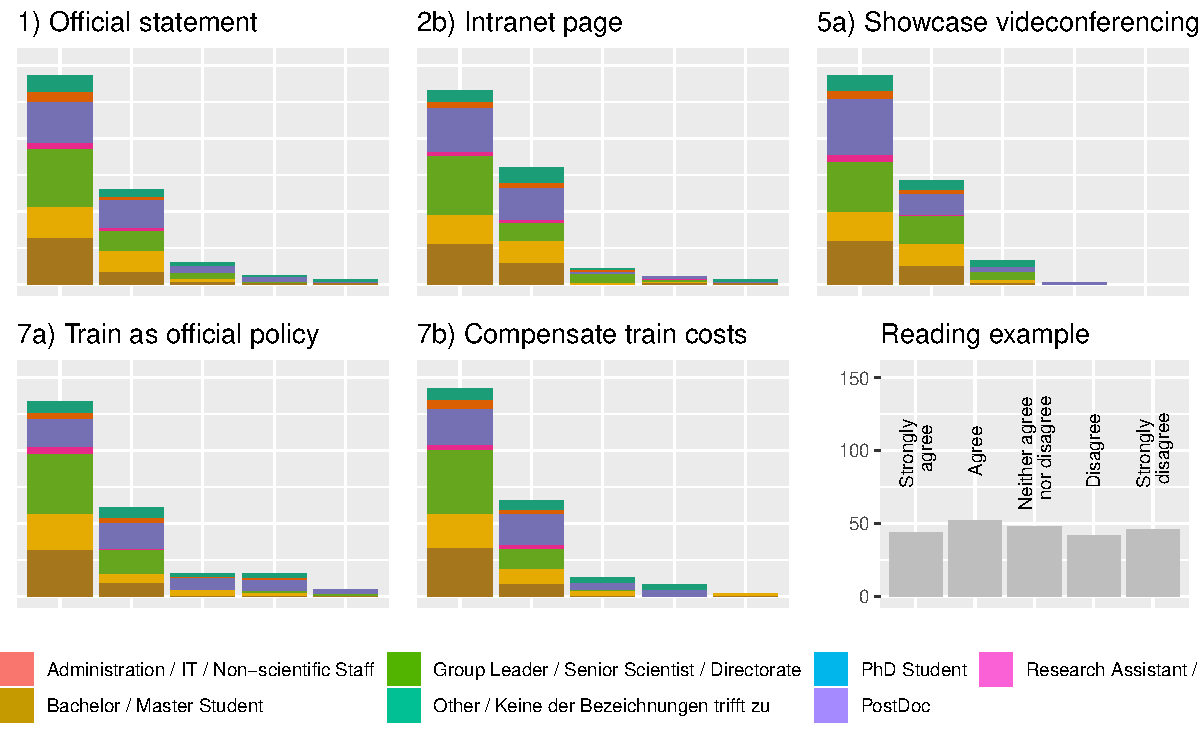
\includegraphics{final_report_files/figure-latex/unnamed-chunk-1-1} \caption[Categorization of measures proposed based on acceptance, expected impact and expected cost]{Categorization of measures proposed based on acceptance, expected impact and expected cost. Each circle represents a measure, sized by expected costs.}\label{fig:unnamed-chunk-1}
\end{figure}

\hypertarget{list-of-measures}{%
\subsection{List of measures}\label{list-of-measures}}

The following list of measures was originally proposed to Eawag
employees for evaluation in the survey conducted by flyaware. It was
elaborated based on gathering a crowd-sourced list of measures first
within a core group and then within the extended flyaware group. To
gather an initial set of measures, initiatives at other institutions,
such as ETH and EPFL were taken into account. We tried to ensure a mix
of regulatory, incentive-based and informational measures.

\hypertarget{official}{%
\section{}\label{official}}

\hypertarget{official-statement-eawag-directive}{%
\subsubsection{\texorpdfstring{\emph{Official Statement (Eawag
Directive)}:}{Official Statement (Eawag Directive):}}\label{official-statement-eawag-directive}}

Eawag officially states that low-carbon transport (e.g.~train) is
preferred over high-carbon transport (e.g.~flying) in an Eawag
directive.

\hypertarget{intranet}{%
\section{}\label{intranet}}

\hypertarget{intranet-page}{%
\subsubsection{\texorpdfstring{\emph{Intranet
page}:}{Intranet page:}}\label{intranet-page}}

Eawag sets up an intranet page on climate friendly mobility. This
webpage will provide useful information on: -International train travel
such as on booking platforms (e.g.~loco2.com, trainline.com and
interrail.eu) that facilitate the booking process of train tickets
within Europe - Video conference training - The compensation system of
CO2 emissions from flying at Eawag

\hypertarget{database}{%
\section{}\label{database}}

\hypertarget{improved-data-base}{%
\subsubsection{\texorpdfstring{\emph{Improved Data
Base}:}{Improved Data Base:}}\label{improved-data-base}}

The Eawag reporting database, which collects data on conference
contributions, supervision of students etc., will be extended to collect
data on mobility behavior. For each international business trip,
information on the following will be collected: -Type of transportation
used (flight, train, bus, etc.) - Purpose of business trip (conference,
project meeting, etc.) - Points of departure and arrival

\hypertarget{role_models}{%
\section{}\label{role_models}}

\hypertarget{highlight-role-models}{%
\subsubsection{\texorpdfstring{\emph{Highlight role
models}:}{Highlight role models:}}\label{highlight-role-models}}

Many Eawag employees already show a high awareness of the impact of
their mobility behavior. The communications department will highlight
Eawag employees who actively reduce their business flights, or avoid
them entirely (e.g.~via intranet, poster exhibition, etc.), in order to
promote role models and to take away the fear that professional
development may suffer by avoiding or reducing business flights.

\hypertarget{appraisal}{%
\section{}\label{appraisal}}

\hypertarget{integrate-in-appraisal-interviews}{%
\subsubsection{\texorpdfstring{\emph{Integrate in appraisal
interviews}:}{Integrate in appraisal interviews:}}\label{integrate-in-appraisal-interviews}}

Reflections on climate friendly mobility become a mandatory part of
yearly appraisal interviews. Supervisors and employees will reflect on
whether a conference and the resultant business flight(s) are truly
necessary to advancing given projects and/or professional development of
the employee.

\hypertarget{showcase_video}{%
\section{}\label{showcase_video}}

\hypertarget{showcasing-video-conferences}{%
\subsubsection{\texorpdfstring{\emph{Showcasing video
conferences}:}{Showcasing video conferences:}}\label{showcasing-video-conferences}}

Eawag promotes the videoconferencing technology by showcasing it during
larger events, such as in Eawag seminars and conferences hosted at
Eawag.

\hypertarget{video_training}{%
\section{}\label{video_training}}

\hypertarget{trainings-for-videoconferencing}{%
\subsubsection{\texorpdfstring{\emph{Trainings for
videoconferencing}:}{Trainings for videoconferencing:}}\label{trainings-for-videoconferencing}}

Regular trainings on the recently installed video conference equipment
will be available for all staff and will be mandatory for all group
leaders.

\hypertarget{video_default}{%
\section{}\label{video_default}}

\hypertarget{default-videoconferencing-for-guests}{%
\subsubsection{\texorpdfstring{\emph{Default videoconferencing for
guests}:}{Default videoconferencing for guests:}}\label{default-videoconferencing-for-guests}}

Eawag makes it official policy that video conferencing is the default
choice for guests who would otherwise need to fly in for meetings and/or
seminars.

\hypertarget{train_travel_policy}{%
\section{}\label{train_travel_policy}}

\hypertarget{train-travel-as-official-policy}{%
\subsubsection{\texorpdfstring{\emph{Train travel as official
policy}:}{Train travel as official policy:}}\label{train-travel-as-official-policy}}

Eawag will recommend and state within the developed directive (see
measure official statement) that flights to destinations that can be
reached within 10 hours by train, or that can be reached using an
overnight train option, should be avoided. The journey will be
considered as working time.

\hypertarget{train_travel_compensate}{%
\section{}\label{train_travel_compensate}}

\hypertarget{compensation-of-train-travel}{%
\subsubsection{\texorpdfstring{\emph{Compensation of train
travel}:}{Compensation of train travel:}}\label{compensation-of-train-travel}}

Possible additional costs for train travel compared to flying
(e.g.~higher ticket price, additional overnight stays, etc.) will be
paid for by Eawag e.g.~by re-allocating funds received through
compensation of flying\#\#\#related CO2 emissions.

\hypertarget{train_firstclasse}{%
\section{}\label{train_firstclasse}}

\hypertarget{finance-first-class-trains}{%
\subsubsection{\texorpdfstring{\emph{Finance first class
trains}:}{Finance first class trains:}}\label{finance-first-class-trains}}

Moreover, first-class train rides might be considered in certain cases
(e.g.~ticket price max. 30\% higher than a standard rate ticket) and
will be financially supported by Eawag (e.g.~by re-allocating funds
received through compensations of flying\#\#\#related CO2 emissions (see
measure 6)) .

\hypertarget{internal_competition}{%
\section{}\label{internal_competition}}

\hypertarget{internal-reduction-targets-per-department}{%
\subsubsection{\texorpdfstring{\emph{Internal reduction targets per
department}:}{Internal reduction targets per department:}}\label{internal-reduction-targets-per-department}}

After having established a database of mobility behavior over three
years (see measure improved database) all departments are requested to
set internal reduction targets, e.g.~a reduction of 20\#\#\#50\% over
the following five years compared to the collected three\#\#\#year
average.

\hypertarget{double_compensation}{%
\section{}\label{double_compensation}}

\hypertarget{double-co2-compensation}{%
\subsubsection{\texorpdfstring{\emph{Double CO2
compensation}:}{Double CO2 compensation:}}\label{double-co2-compensation}}

To further support climate friendly travel options, the CO2 compensation
fee for all flights will be doubled.

\hypertarget{compensate_all_flights}{%
\section{}\label{compensate_all_flights}}

\hypertarget{compensate-all-flights}{%
\subsubsection{\texorpdfstring{\emph{Compensate all
flights}:}{Compensate all flights:}}\label{compensate-all-flights}}

All flights, independent of the funding source, are collected in the
reporting database (see measure improved database). Hence, even flights
paid for through external funding (e.g.~invitations by other research
institutes, universities etc.) - which haven't previously been
considered - will also be compensated.

\hypertarget{internal_comp_xmas}{%
\section{}\label{internal_comp_xmas}}

\hypertarget{internal-competition-highlight-at-xmas}{%
\subsubsection{\texorpdfstring{\emph{Internal competition, highlight at
Xmas}:}{Internal competition, highlight at Xmas:}}\label{internal-competition-highlight-at-xmas}}

Results of the mobility behavior collected in the reporting database
(see measure improved database) will be presented at the Eawag Christmas
party. Departments with the largest relative reduction of CO2 emissions
related to their mobility behavior will be highlighted and awarded
(e.g.~by a department excursion sponsored by Eawag) every year.

\hypertarget{overseas_restriction}{%
\section{}\label{overseas_restriction}}

\hypertarget{restrictions-of-overseas-flights}{%
\subsubsection{\texorpdfstring{\emph{Restrictions of Overseas
Flights}:}{Restrictions of Overseas Flights:}}\label{restrictions-of-overseas-flights}}

Overseas flights cause by far the largest amount of CO2 emissions among
Eawag business flights. Therefore, Eawag will restrict the number of
overseas flights (except for field work): - Group Leaders, Department
Heads and the Directorate: 1 overseas flight within 2 years - PhD
students and Postdocs: 1 overseas flight within PhD / Postdoc project
period - Other staff: 1 overseas flight within 4 years (comparable to
length of PhD project)

\hypertarget{internal_cap}{%
\section{}\label{internal_cap}}

\hypertarget{internal-cap}{%
\subsubsection{\texorpdfstring{\emph{Internal
cap}:}{Internal cap:}}\label{internal-cap}}

Every department gets an annual CO2 emissions budget (e.g.~based on the
average CO2 emissions patterns from previous years, as collected in the
reporting database (see measure 3)), which can be allocated and traded
(e.g.~in the shape of certificates) among departments and individuals.

\hypertarget{progressive_cap}{%
\section{}\label{progressive_cap}}

\hypertarget{progressive-cap}{%
\subsubsection{\texorpdfstring{\emph{Progressive
cap}:}{Progressive cap:}}\label{progressive-cap}}

The cap could be progressive over time: increasing slowly for the first
few years and then more quickly later, so that departments can plan
ahead, prepare and adjust themselves to the updated regulations.

\hypertarget{list-of-flyaware-members}{%
\subsection{List of flyaware members}\label{list-of-flyaware-members}}

(alphabetisch)

\bibliography{skeleton.bib}



\end{document}
